\documentclass[a4paper, 12pt, final, garamond]{book}
\usepackage{cours-preambule}

\raggedbottom

\makeatletter
\renewcommand{\@chapapp}{M\'ecanique -- chapitre}
\makeatother

% \toggletrue{student}
% \HideSolutionstrue
\toggletrue{corrige}
\renewcommand{\mycol}{black}
% \renewcommand{\mycol}{gray}

\begin{document}
\setcounter{chapter}{2}

\chapter{\cswitch{Correction du TD}{TD entra\^inement~: mouvements courbes}}
\resetQ
\section{Glissade d'un pingouin sur un igloo}

\enonce{%
	\noindent
	\begin{minipage}{0.70\linewidth}
		Un pingouin, assimilable à un point matériel M de masse $m$ décide de faire
		du toboggan. Il s'élance sans vitesse initiale du sommet A d'un igloo
		voisin, assimilable à une demi sphère $S$ de rayon $R$ et de centre O, posée
		sur un plan horizontal $\Pi$. On considère que le glissement s'effectue sans
		frottement dans le plan vertical ($x$O$z$).
	\end{minipage}
	\hfill
	\begin{minipage}{0.25\linewidth}
		\begin{center}
			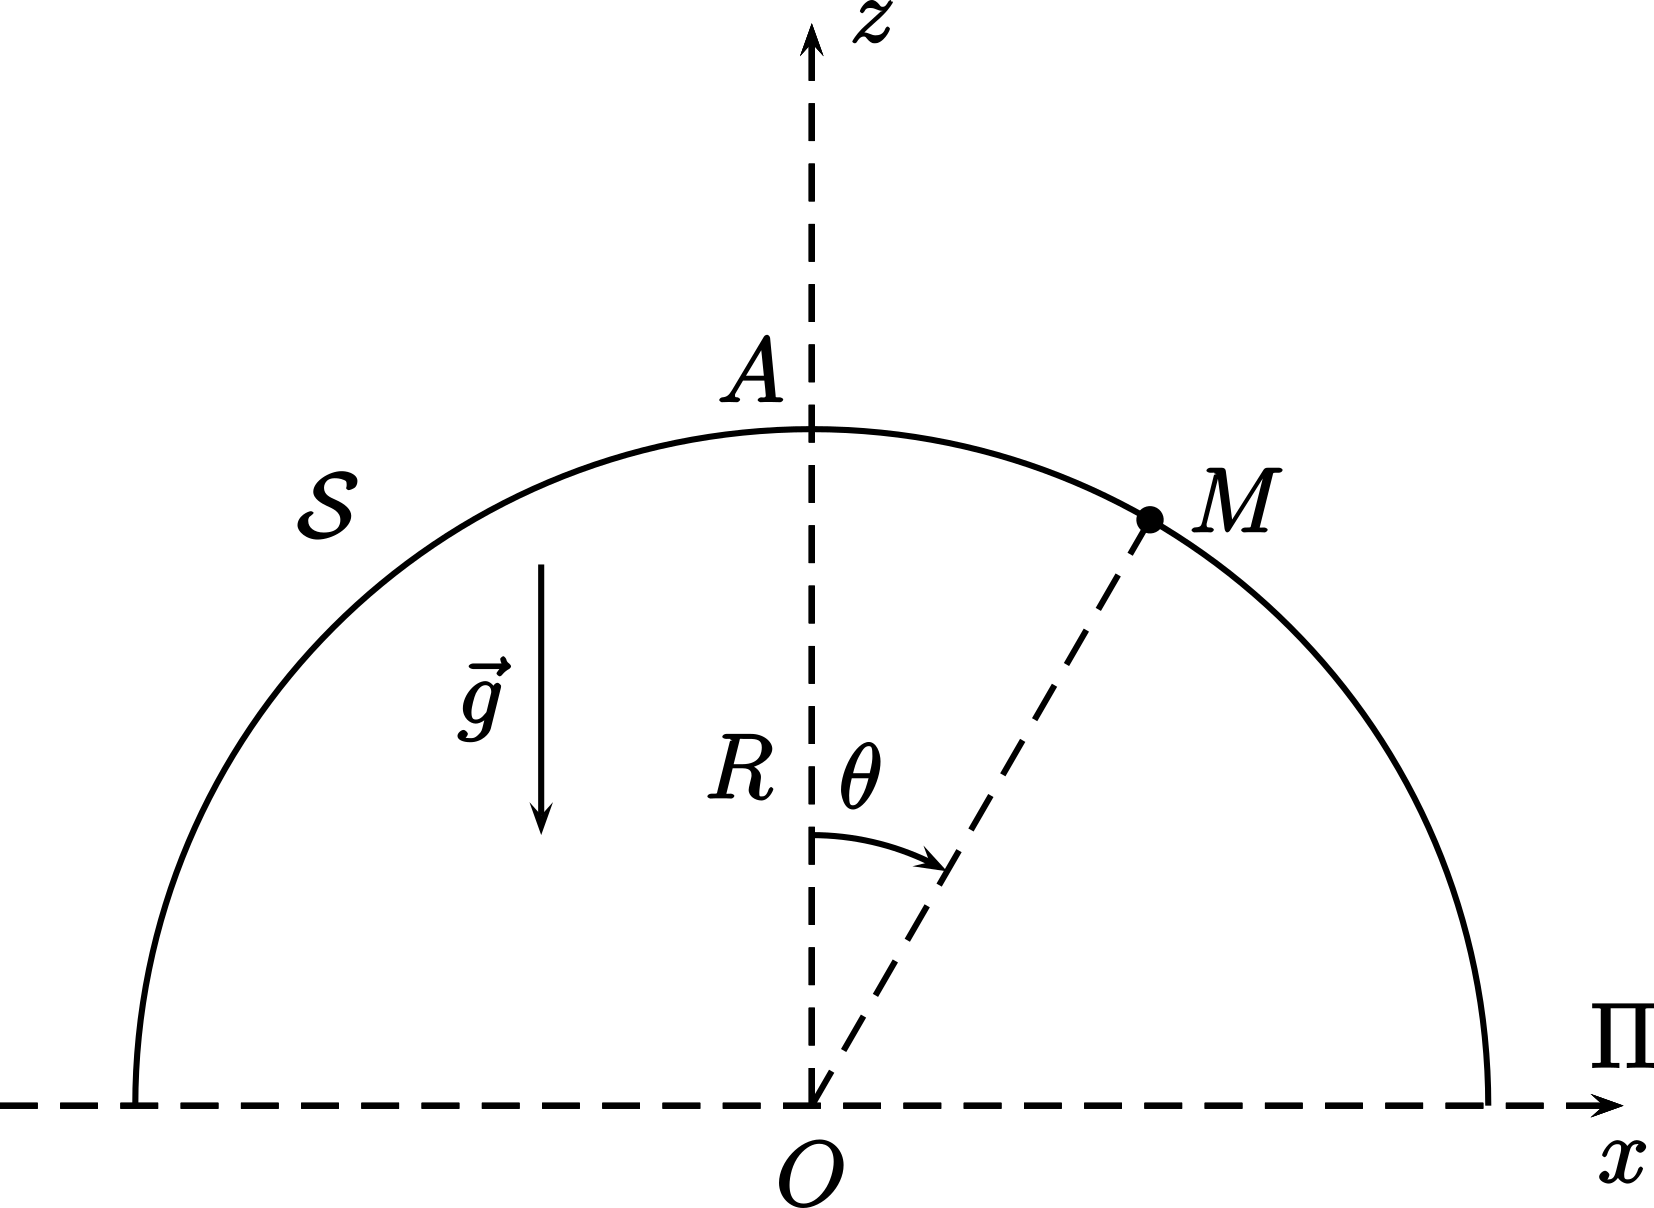
\includegraphics[width=\linewidth]{igloo-plain}
		\end{center}
	\end{minipage}
}

\QR{%
	Appliquer le PFD au pingouin pour en déduire deux équations
	différentielles portant sur l'angle $\tt$. Identifier l'équation du
	mouvement qui permet de déterminer $\tt(t)$. Quelle information l'autre
	information contient-elle~?
}{%
	\begin{itemize}[label=$\diamond$, leftmargin=10pt]
		\bitem{Système~:} \{pingouin\}
	\end{itemize}
	\begin{minipage}{0.70\linewidth}
		\begin{itemize}[label=$\diamond$, leftmargin=10pt]
			\bitem{Référentiel~:} $\Rc\ind{sol}$ supposé galiléen
			\bitem{Repère~:} $(\Or, \ur, \ut)$ avec $\ut$ \textbf{dans le sens de
				$\tt$}
			\bitem{Repérage~:}
			\vspace*{-12pt}
			\begin{align*}
				\OM(t) & = R\ur                 \\
				\vf(t) & = R\tp\ut              \\
				\af(t) & = R\tpp\ut - R\tp^2\ur
			\end{align*}
		\end{itemize}
	\end{minipage}
	\hfill
	\begin{minipage}{0.25\linewidth}
		\begin{center}
			\hspace*{-3cm}
			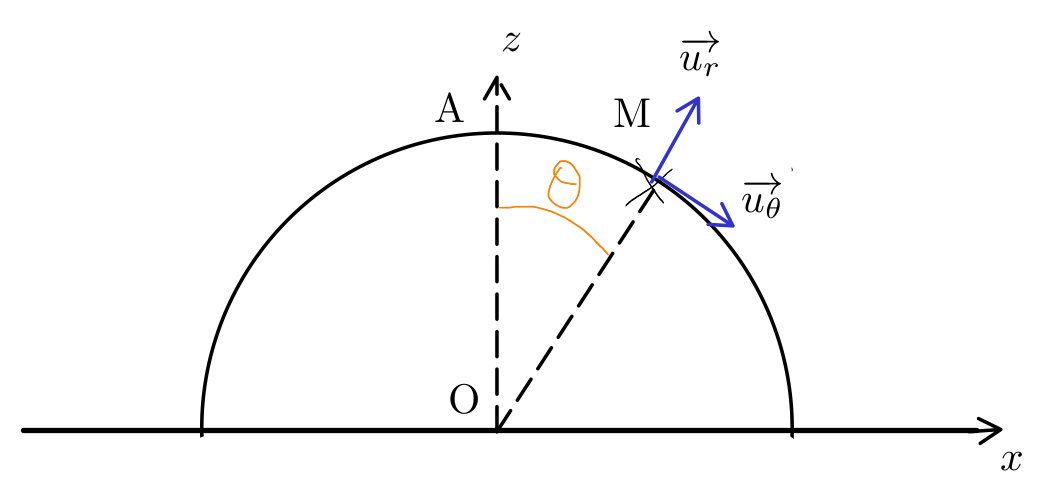
\includegraphics[width=1.8\linewidth]{igloo_corr}
		\end{center}
	\end{minipage}
	\vspace*{12pt}
	\begin{itemize}[label=$\diamond$, leftmargin=10pt]
		\bitem{Origine et instant initial~:}
		\begin{gather*}
			\OM(0) = \vv{\rm OA} \Ra \tt(0) = 0\\
			\vf(0) = \of \Ra \tp(0) = 0
		\end{gather*}
		\bitem{BDF~:}
		\[
			\begin{array}{ll}
				\textbf{Poids}    & \Pf = mg(-\cos\tt\ur +\sin\tt\ut) \\
				\textbf{Réaction} & \Rf = R_N\ur
			\end{array}
		\]
		\item \leftcenters{\textbf{PFD~:}}{
			      $\DS
				      m\af = \Pf + \Rf
				      \Lra
				      \mqty(-mR\tp^2\\mR\tpp) = \mqty(-mg\cos\tt+R_N\\mg\sin\tt)
			      $}
		      \begin{empheq}[box=\fbox, left=\Lra\empheqlbrace]{align}
			      \label{eq:pinga}
			      R_N  & = mg\cos\tt - mR\tp^2\\
			      \label{eq:pingb}
			      \tpp & = \frac{g}{R}\sin\tt
		      \end{empheq}
	\end{itemize}
	L'équation du mouvement est celle qui donne l'équation d'oscillateur
	harmonique aux petits angles, et qu'on a déjà utilisée en cours sur le
	pendule, et linéaire en $\tt$~: l'équation~\eqref{eq:pingb}.
	L'équation~\eqref{eq:pinga} contient l'information sur le contact à
	l'igloo.
}
\QR{%
	En multipliant l'équation du mouvement par $\tp$ et en intégrant sur
	$t$, montrer que
	\[\tp^2 = \frac{2g}{R}(1-\cos\tt)\]
}{%
	En prenant~\eqref{eq:pingb}$\times\tp$, on a
	\begin{align*}
		\tpp\tp
		              & = \frac{g}{R} \tp\sin\tt
		\\\Lra
		\dv{t}(\frac{1}{2}\tp^2)
		              & = \frac{g}{R} \dv{t}(-\cos\tt)
		\\\Lra
		\frac{1}{2}\int_{t=0}^{t} \dv{\tp^2}{t}\dt
		              & = \frac{g}{R}\int_{t=0}^{t} \dv{(-\cos\tt)}{t}\dt
		\\\Lra
		\frac{1}{2} \left[ \tp^2 \right]_{t=0}^{t}
		              & = \frac{g}{R} \left[ -\cos\tt \right]_{t=0}^{t}
		\\\Lra
		\Aboxed{\tp^2 & = \frac{2g}{R}(1-\cos\tt)}
		\qed
	\end{align*}
}
\QR{%
	En déduire la norme de la force de réaction de l'igloo.
}{%
	En reprenant~\eqref{eq:pinga}, on peut remplacer $\tp^2$~:
	\begin{align*}
		R_N         & = mg\cos\tt -m\cancel{R}\frac{2g}{\cancel{R}}(1-\cos\tt)
		\\\Lra
		\Aboxed{R_N & = mg(3\cos\tt -2)}
	\end{align*}
}
\QR{%
	Le pingouin décolle-t-il du toit de l'igloo avant d'atteindre le sol~?
	Si oui, pour quel angle~?
}{%
	La condition de support d'un solide est $R_N > 0$~: le pingouin
	décolle du support si la force de réaction est nulle, soit $R_N = 0$.
	Or,
	\begin{align*}
		R_N          & = 0
		\\\Lra
		3\cos\tt - 2 & =0
		\\\Lra
		\Aboxed{\tt  & = \arccos(\frac{2}{3})}
	\end{align*}
	Une application numérique donne \fbox{$\tt = \ang{48.2}$}.
}

\resetQ
\section{Course de F1}
\enonce{%
	\noindent
	\begin{minipage}{0.70\linewidth}
		Lors des essais chronométrés d'un grand prix, Fernando \textsc{Alonso}
		(point A) et Jenson \textsc{Button} (point B) arrivent en ligne droite et
		coupent l'axe $\D$ au même instant de leur parcours. Ils prennent cependant
		le virage de deux façons différentes~:
		\bigbreak
		\begin{itemize}
			\item \textsc{Alonso} suit une trajectoire circulaire de rayon $R_A =
				      \SI{90.0}{m}$~;
			\item \textsc{Button} choisit une trajectoire de rayon $R_B = \SI{75.0}{m}$.
		\end{itemize} \bigbreak
		On cherche à déterminer quelle est la meilleure trajectoire, c'est-à-dire
		lequel des deux pilote gagne du temps par rapport à l'autre à la sortie du
		virage.
	\end{minipage}
	\hfill
	\begin{minipage}{0.25\linewidth}
		\begin{center}
			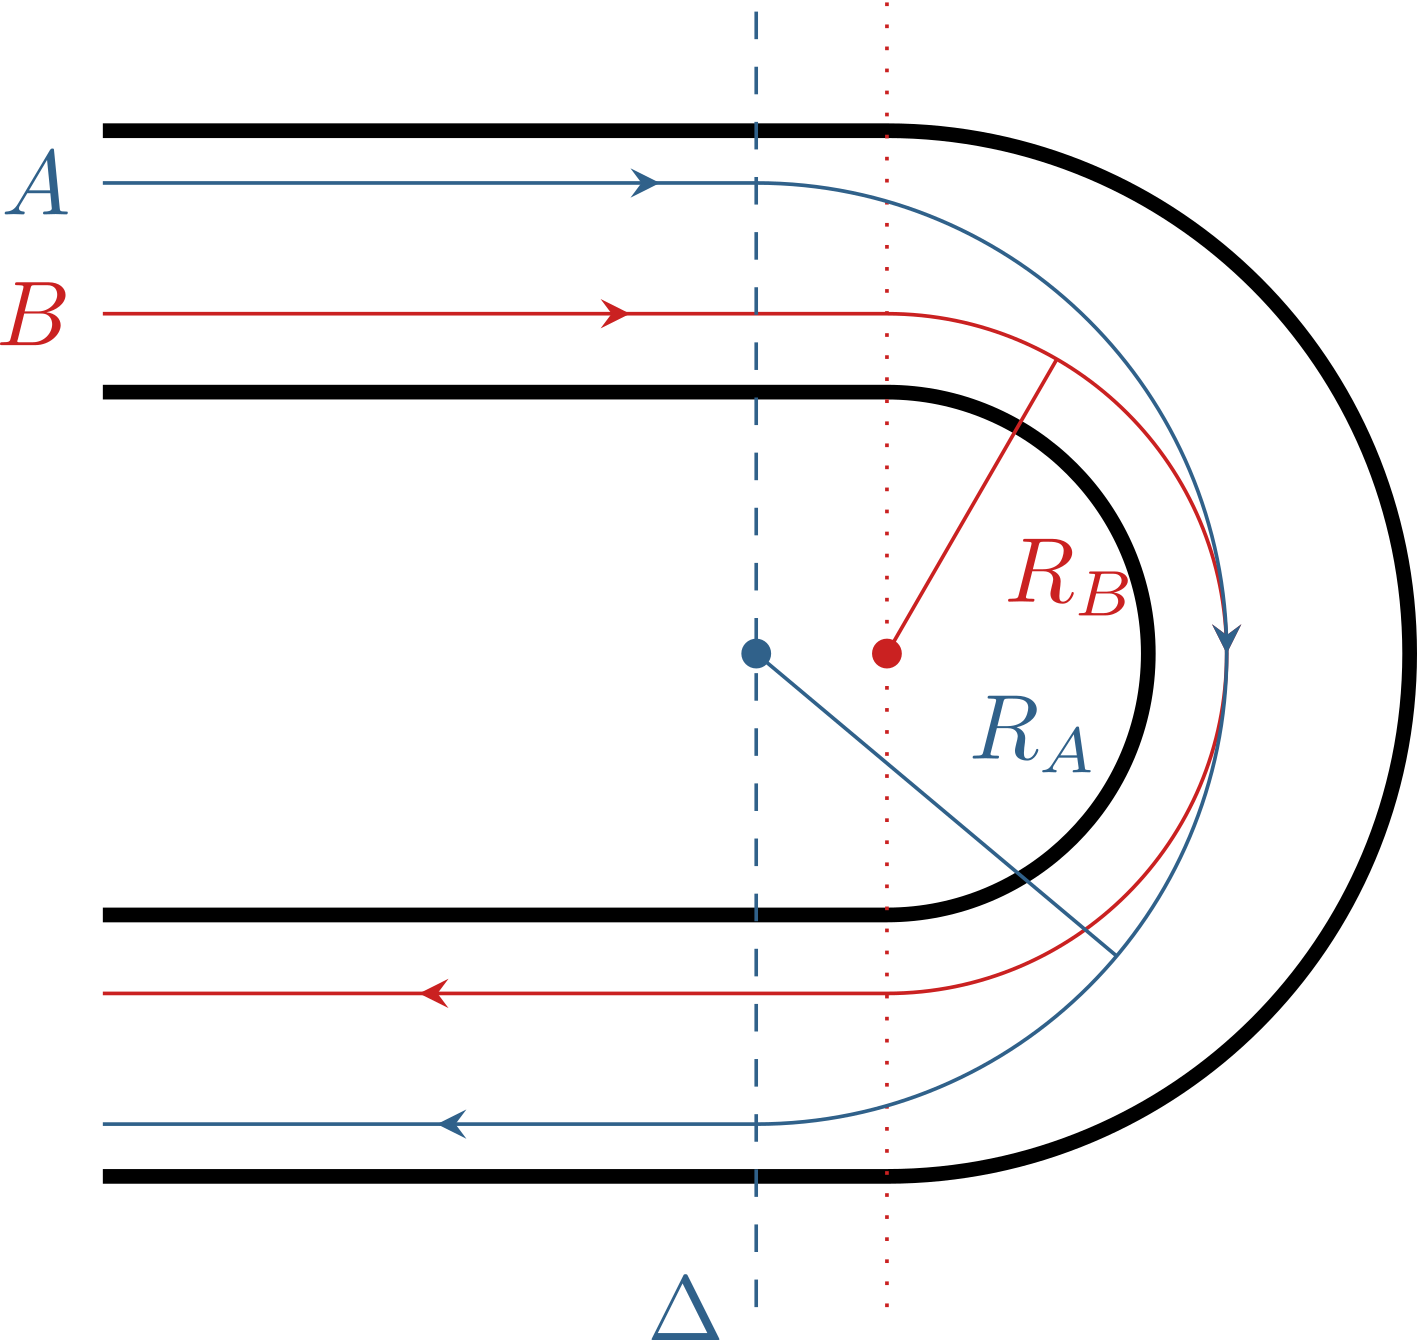
\includegraphics[width=\linewidth]{F1_plain}
		\end{center}
	\end{minipage}
}

\QR{%
	Déterminer les distances $D_A$ et $D_B$ parcourues par les deux
	pilotes entre leurs deux passages par l'axe $\D$. Que peut-on conclure~?
}{%
	La voiture A d'\textsc{Alonso} entame son virage dès qu'elle passe par
	l'axe $\D$, et parcourt un demi-cercle de longueur
	\[\boxed{D_A = \pi R_A = \SI{283}{m}}\]
	En revanche, la voiture B de \textsc{Button} continue en ligne droite
	sur une distance $R_A-R_B$ avant d'entamer son virage, et parcourt de
	nouveau la même distance en ligne droite avant la sortie du virage.
	Ainsi,
	\[\boxed{D_B = 2(R_1-R_2) + \pi R_B = \SI{266}{m}}\]
	La voiture B parcourt moins de distance que la voiture A, mais
	\textbf{il est impossible d'en conclure quoi que ce soit} puisqu'on ne
	sait pas si les deux trajectoires sont parcourues à la même vitesse.
}
\QR{%
	Pour simplifier, on imagine que les deux voitures roulent à des
	vitesse $v_A$ et $v_B$ constantes entre leurs deux passages par l'axe
	$\D$. Déterminer ces vitesses, sachant que l'accélération des voitures
	doit rester inférieur à \SI{0.8}{g} sous risque de dérapage. Les
	calculer numériquement.
}{%
	Lorsqu'elles sont sur la partie circulaire de leur trajectoire,
	parcourue à vitesse constante (en norme), l'accélération (en norme) des
	voitures vaut
	\[a = \frac{v^2}{R} = \num{0.8}g\]
	puisque les pilotes prennent tous les risques. Ainsi,
	\[
		\boxed{v_A = \sqrt{aR_A} = \SI{26.6}{m.s^{-1}}}
		\qet
		\boxed{v_B = \sqrt{aR_B} = \SI{24.3}{m.s^{-1}}}
	\]
}
\QR{%
	Conclure quant à la meilleure trajectoire des deux.
}{%
	Calculons le temps mis par chacun des pilotes pour passer le virage.
	On sait que
	\[\Dt = \frac{D}{v}\]
	d'où les résultats
	\[
		\boxed{\Dt_A = \SI{10.6}{s}}
		\qet
		\boxed{\Dt_B = \SI{10.9}{s}}
	\]
	Finalement, \textsc{Alonso} va plus vite que \textsc{Button} pour
	parcourir le virage~: \textbf{la meilleure trajectoire est la meilleure
		des deux}. À ne pas tenter en vérifiant chez soi, mais de quoi briller
	sur Mario Kart…?
}

\resetQ
\section{Entraînement d'une spationaute}

\noindent
\enonce{%
	\begin{minipage}{0.70\linewidth}
		Une spationaute doit subir différents tests d'aptitude aux vols spatiaux,
		notamment le test des accélérations. Pour cela, on l'installe dans une
		capsule de centre O, fixée au bout d'un bras métallique horizontal dont
		l'autre extrémité est rigidement liée à un arbre de rotation vertical $\D$.
		La longueur du bras est notée $L$. On assimilera la spationaute au point
		matériel S. \bigbreak
	\end{minipage}
	\hfill
	\begin{minipage}{0.25\linewidth}
		\begin{center}
			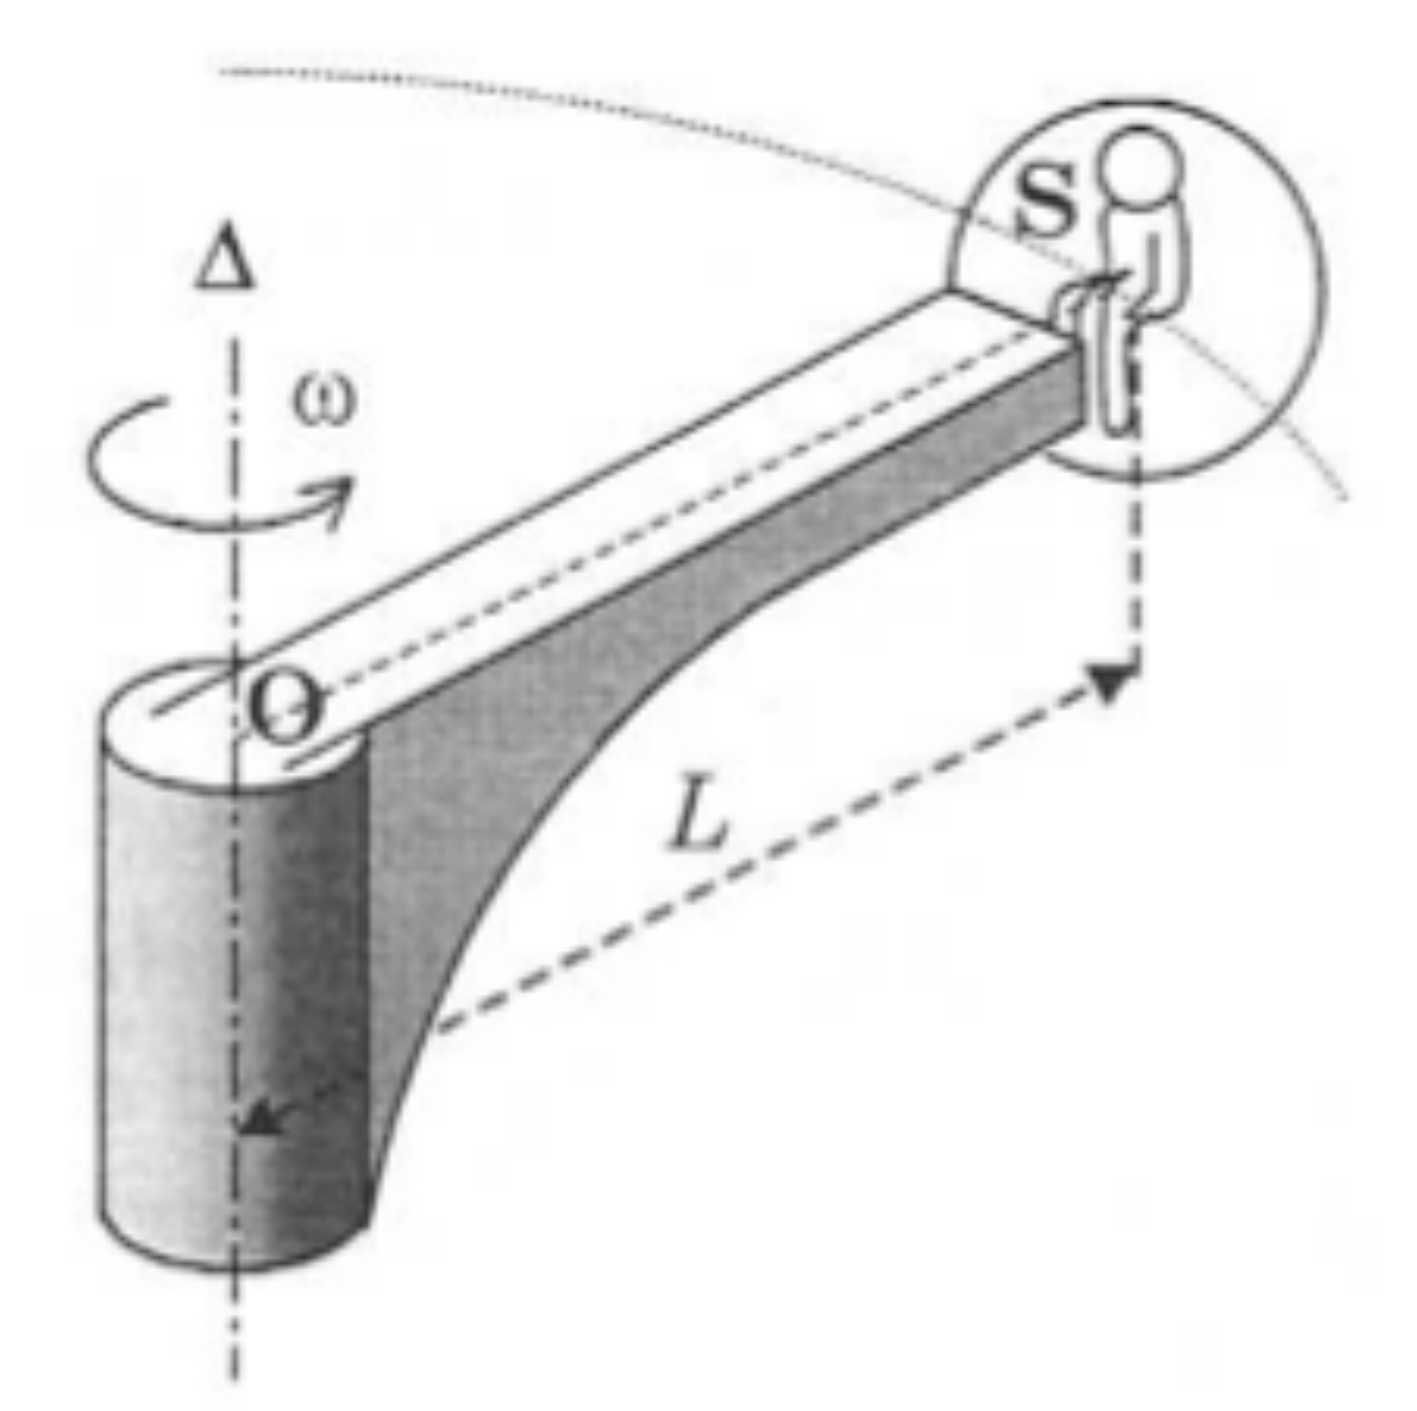
\includegraphics[width=\linewidth]{centri_spat-plain}
		\end{center}
	\end{minipage}
	L'ensemble \{capsule + bras + arbre\} est mis en rotation avec un vitesse
	angulaire croissant progressivement selon la loi
	\[\w(t) = \w_0(1-\exp^{-t/\tau})\]
	avec $\w_0$ la vitesse angulaire nominale du simulateur, et $\tau$ un temps
	caractéristique. On donne $L = \SI{10.0}{m}$ et $g = \SI{9.81}{m.s^{-2}}$.
}
\bigbreak
\QR{%
	Établir proprement le système d'étude.
}{%
	\begin{itemize}[label=$\diamond$] %, leftmargin=10pt]
		\bitem{Système~:} \{spationaute\}
		\bitem{Référentiel~:} référentiel du laboratoire, supposé galiléen
		\bitem{Repère~:} $(\Or,\ur,\ut)$ avec $\ut$ selon le sens de rotation
	\end{itemize}
	\begin{minipage}{0.60\linewidth}
		\begin{itemize}[label=$\diamond$] %, leftmargin=10pt]
			\bitem{Repérage~:}
			\begin{align*}
				\vv{\rm OS}(t) & = L\ur                   \\
				\vf_S(t)       & = L\w\ut                 \\
				\af_S(t)       & = L\dot{\w}\ut -L\w^2\ur
			\end{align*}
		\end{itemize}
	\end{minipage}
	\hfill
	\begin{minipage}{0.35\linewidth}
		\begin{center}
			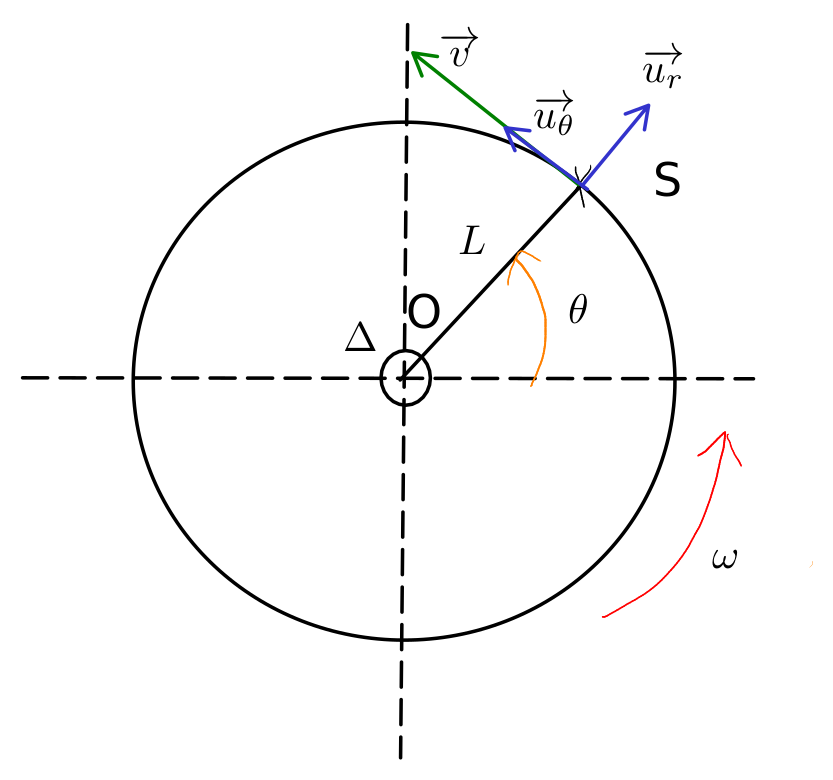
\includegraphics[scale=0.15]{spationaute_corr}
		\end{center}
	\end{minipage}
}
\QR{%
	À partir de quelle durée peut-on supposer que le mouvement est
	circulaire et uniforme~? Que deviennent les expressions des vecteurs
	vitesse et accélération dans ce cas~? Calculer alors la norme de
	l'accélération subie par la spationaute.
}{%
	Au bout de quelques $\tau$, $\w(t) = \w_0$ et le mouvement sera
	circulaire uniforme. Les vecteurs vitesse et accélération deviennent~:
	\begin{empheq}[box=\fbox, left=\empheqlbrace]{align*}
		\vf_S(t) &= L\w_0\ut\\
		\af_S(t) &= -L\w_0{}^2\ur
	\end{empheq}
	La norme de l'accélération subie est alors \fbox{$\norm{\af_S} =
			L\w_0{}^2$}.
}
\QR{%
	Quelle doit être la valeur de $\w_0$ pour que l'accélération atteigne
	\SI{10}{g} lors du régime de rotation uniforme~? On donnera le résultat
	en tours par second.
}{%
	\begin{gather}
		a_S = 10g \Ra \boxed{\w_0 = \sqrt{\frac{10g}{L}}}
		\qavec
		\left\{
		\begin{array}{rcl}
			g & = & \SI{9.81}{m.s^{-2}} \\
			L & = & \SI{10.0}{m}
		\end{array}
		\right.\\
		\AN
		\boxed{\w_0 = \SI{3.13}{rad.s^{-1}} \approx \SI{0.50}{tour.s^{-1}}}
	\end{gather}
	\begin{tcb}(odgr){Ordres de grandeurs}
		\begin{itemize}[label=$\diamond$]
			\item Accélération latérale en F1~: \SIrange{4}{5}{g}~;
			\item Accélération latérale en avion de chasse~: \SIrange{9}{10}{g}
			      pendant quelques secondes max~;
			\item Accélération verticale, éjection d'un avion de chasse~: $\approx
				      \SI{20}{g}$ (interdiction de vol après 2 utilisation du siège
			      éjectable à cause – notamment – du tassement des vertèbres)~;
			\item Accélération négative frontale en accident de voiture~:
			      \SIrange{40}{60}{g}~! Même sans choc physique, une telle
			      décélération cause des hémorragies internes à cause des organes
			      internes percutant les os. Soyez prudent-es.
		\end{itemize}
	\end{tcb}
}

\resetQ
\section{Anneau sur une tige en rotation}

\noindent
\enonce{%
	\begin{minipage}{0.70\linewidth}
		On considère un petit anneau M de masse $m$ considéré comme ponctuel, soumis
		à la pesanteur et susceptible de se déplacer sans frottement le long d'une
		tige OA horizontale dans le plan ($x$O$y$), de longueur $\ell$, effectuant
		des mouvements de rotation caractérisés par une vitesse angulaire $\w$
		constante autour d'un axe fixe vertical $\D$ passant par son extrémité O. Le
		référentiel lié au laboratoire est considéré comme galiléen. On considère~:
		\bigbreak
		\begin{itemize}
			\item le repère cartésien $(\Or,\ex,\ey,\ez)$ fixe dans le référentiel
			      du laboratoire et associé aux axes $x$, $y$ et $z$~;
			\item la base cylindrique locale $(\er,\et,\ez)$ associée au point M.
		\end{itemize}
		\bigbreak
	\end{minipage}
	\hfill
	\begin{minipage}{0.25\linewidth}
		\begin{center}
			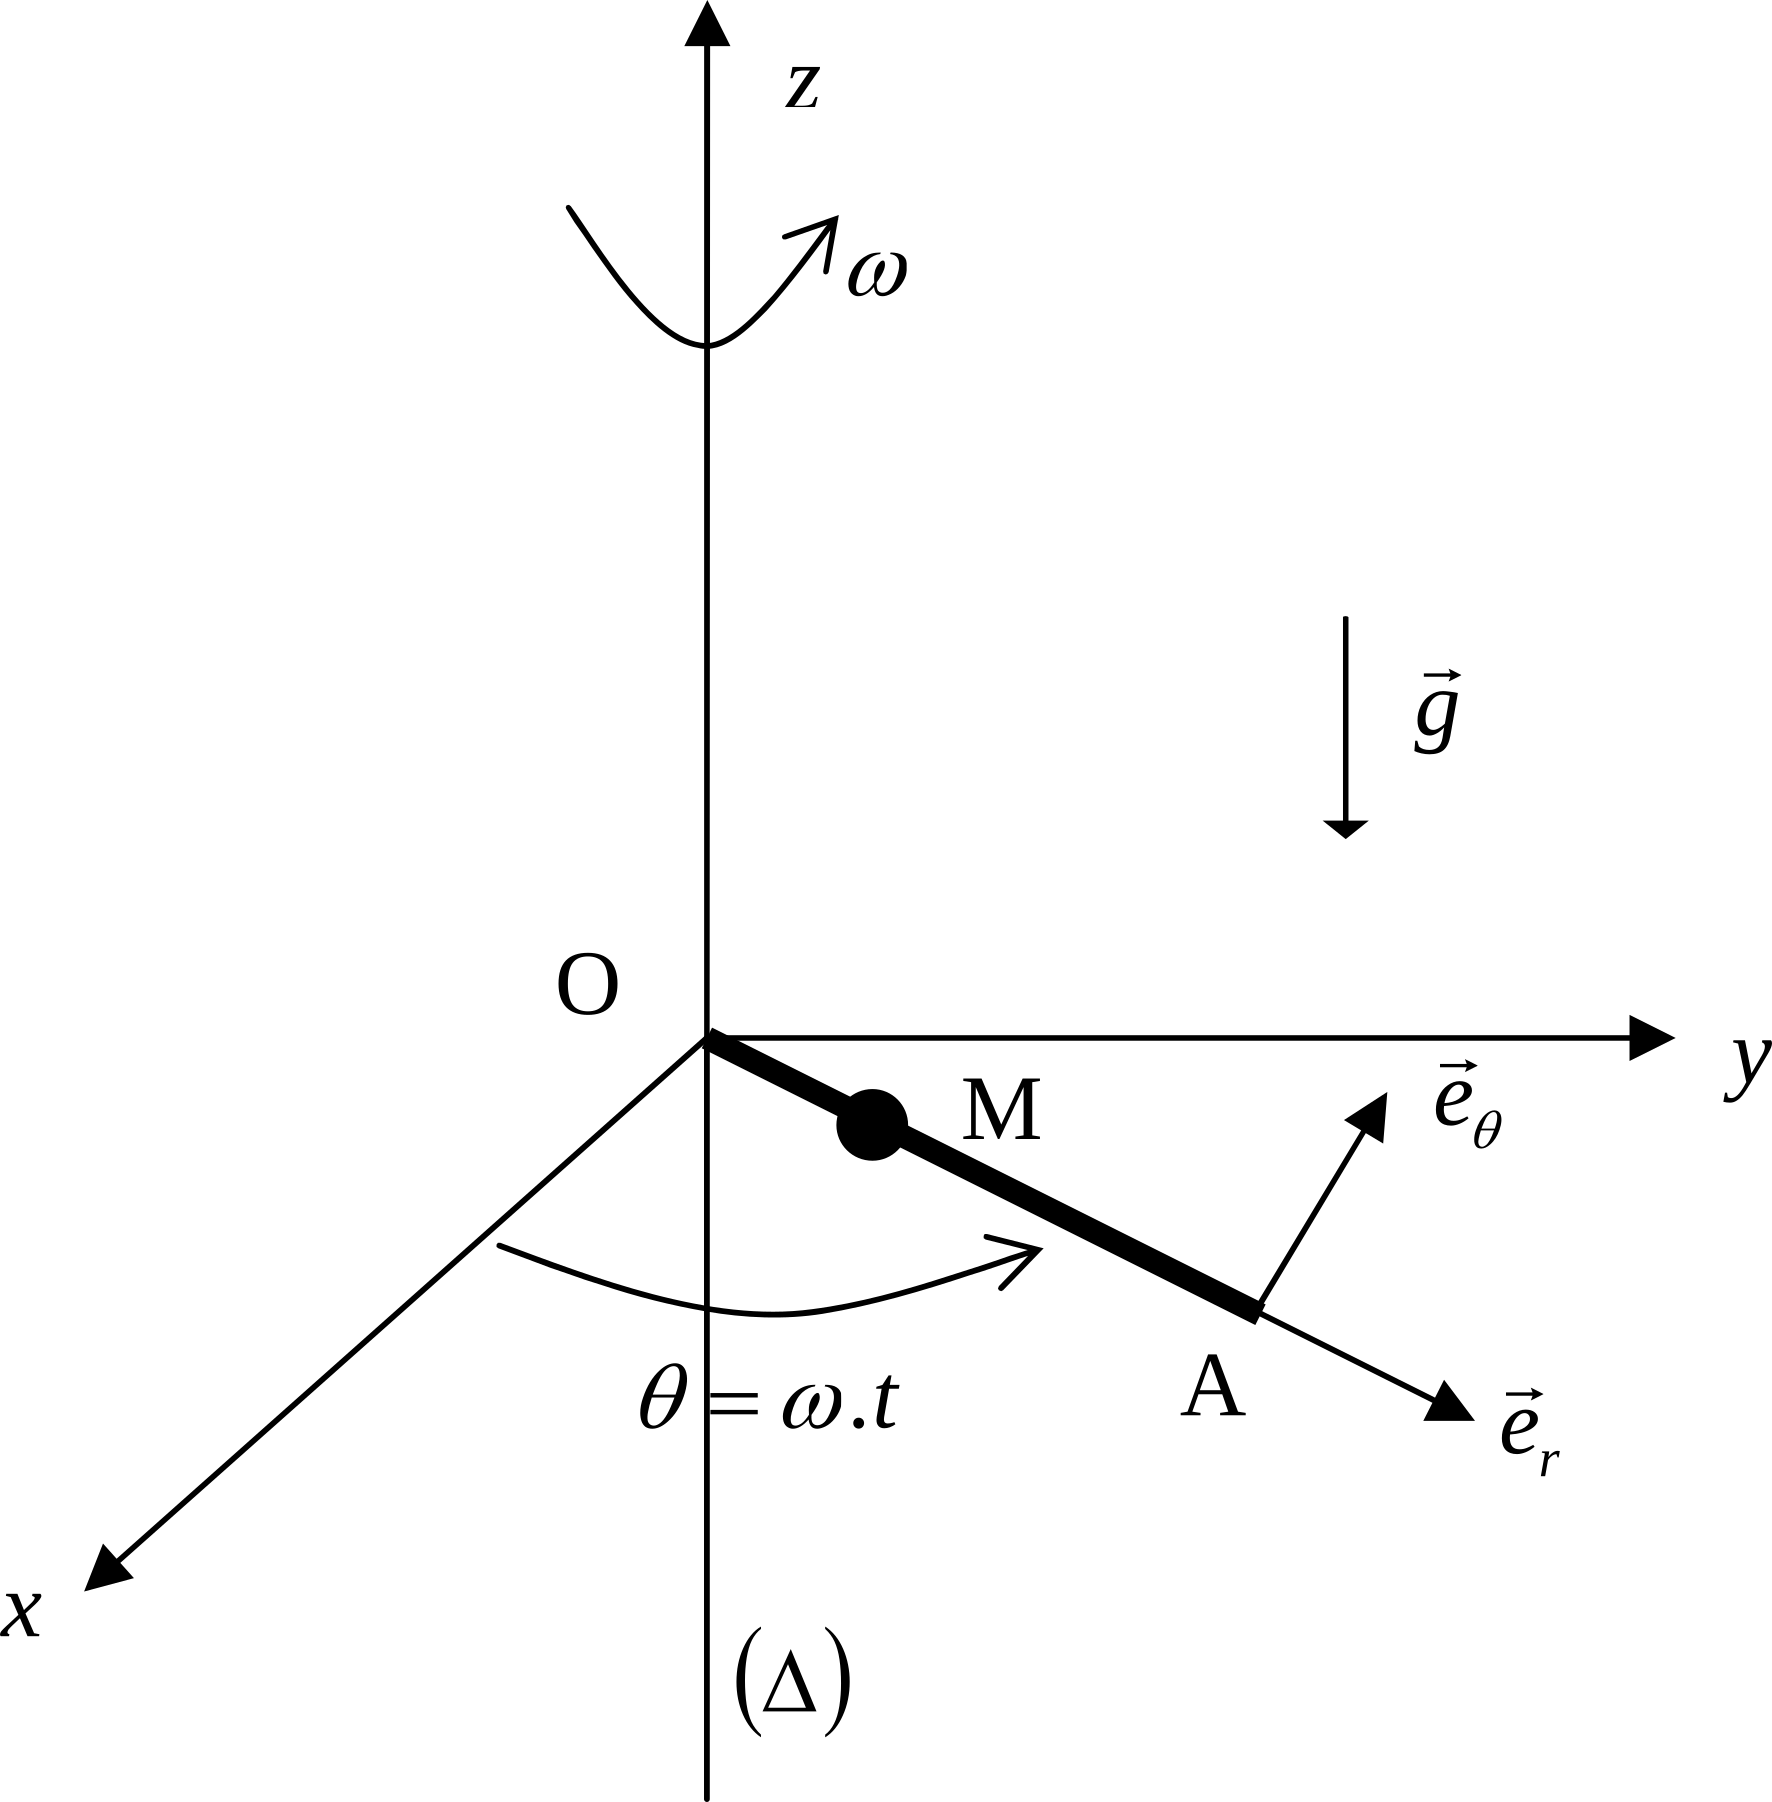
\includegraphics[width=\linewidth]{anneau_tige_rot-plain}
		\end{center}
	\end{minipage}
	L'anneau est libéré sans vitesse initiale par rapport à la tige, à une
	distance $r_0$ du point O (avec $r_0 < \ell$). On repère la position de
	l'anneau sur la tige par la distance $r = \OMr$ entre le point O et l'anneau
	M.
}
\QR{%
	Faire un bilan des forces agissant sur l'anneau en les projetant dans
	la base $(\er,\et,\ez)$. En appliquant le
	principe fondamental de la dynamique, établir l'équation différentielle
	vérifiée par $r(t)$.
}{%
	\begin{minipage}[t]{0.60\linewidth}
		\begin{itemize}[label=$\diamond$, leftmargin=10pt]
			\bitem{Système~:} \{anneau\} point matériel M de masse $m$
			\bitem{Référentiel~:} terrestre supposé galiléen
			\bitem{Repère~:} cylindrique $(\Or,\er,\et,\ez)$
			\bitem{Repérage~:}
			\begin{align*}
				\OM & = r\er                                        \\
				\vf & = \rp\er + r\tp\et                            \\
				    & = \rp\er + r\w\et                             \\
				\af & = \rpp\er + \rp\tp\et + \rp\w\et - r\w^2\er +
				\underbracket[0.4pt]{\of}_{\dot{\w}=0}              \\
				    & = (\rpp -r\w^2)\er +2r\w\et
			\end{align*}
		\end{itemize}
	\end{minipage}
	\hfill
	\begin{minipage}[t]{0.35\linewidth}
		~
		%\vspace*{6cm}
		\begin{center}
			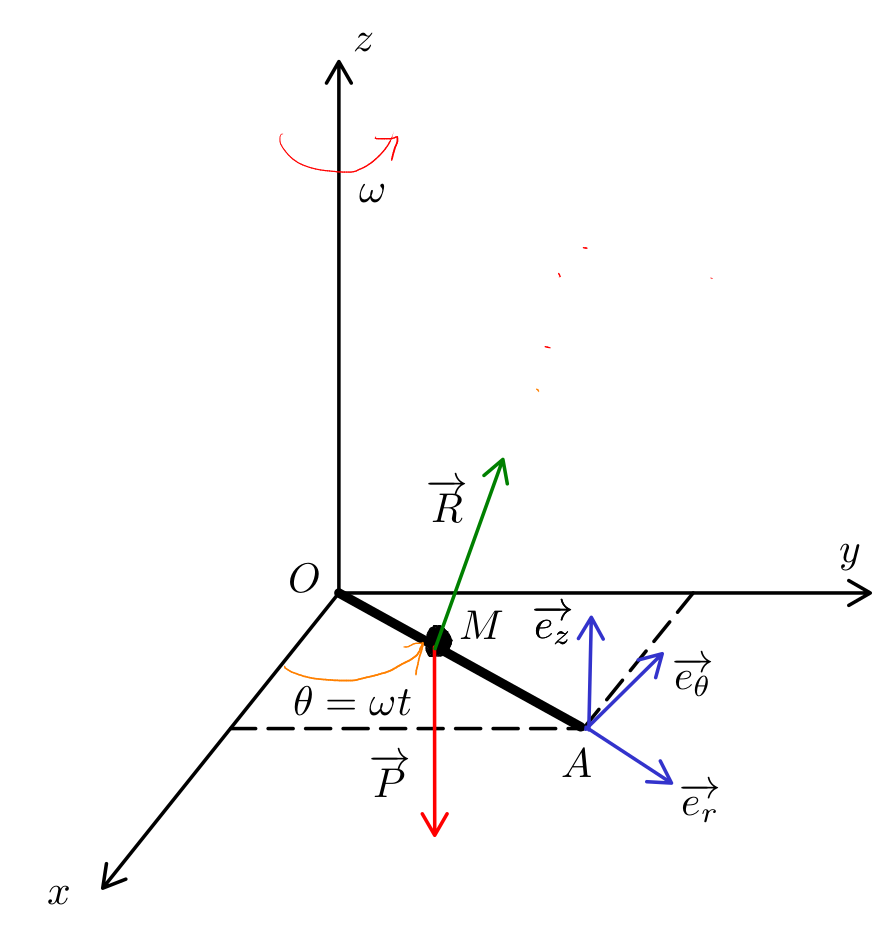
\includegraphics[scale=.18]{tige_rot_corr}
		\end{center}
	\end{minipage}
	\begin{itemize}[label=$\diamond$, leftmargin=10pt]
		\bitem{Conditions initiales~:}
		\[
			r(0) = r_0
			\qet
			\vf(0) = \of \Ra \rp(0) = 0
		\]
		\bitem{BDF~:} pas de frottements donc pas de composante sur $\er$~:
		\[
			\begin{array}{ll}
				\textbf{Poids}            & \Pf = m\gf = -mg\ez     \\
				\textbf{Réaction support} & \Rf = R_\tt\et + R_z\ez
			\end{array}
		\]
		\bitem{PFD~:}
		\begin{gather*}
			m\af = \Pf + \Rf
			\Lra
			\left\{
			\begin{aligned}
				m(\rpp-r\w^2) & = 0         \\
				2m\rp\w       & = R_\tt     \\
				0             & = -mg + R_z
			\end{aligned}
			\right.
		\end{gather*}
		\begin{empheq}[box=\fbox, left=\Lra\empheqlbrace]{align}
			\label{eq:tigerota}
			\Aboxed{
				\rpp - \w r &= 0
			}\\
			\label{eq:tigerotb}
			R_\tt &= 2m\rp\w\\
			\label{eq:tigerotc}
			R_z &= mg
		\end{empheq}
	\end{itemize}
}
\QR{%
	Intégrer cette équation différentielle en prenant en compte les
	conditions initiales définies précédemment, et déterminer la solution
	$r(t)$ en fonction de $r_0$, $\w$ et $t$.
}{%
	On résout~\eqref{eq:tigerota} avec l'équation caractéristique~:
	\begin{align*}
		\rpp -\w^2r & = 0
		\\\Ra
		s^2 - \w^2  & = 0
		\\\Lra
		s^2         & = \w^2
		\\\Lra
		\Aboxed{s   & = \pm\w}
	\end{align*}
	On a donc des solutions de la forme
	\begin{gather*}
		r(t) = A\exr^{\wt} + B\exr^{-\wt}
		\shortintertext{Or, avec les CI~:}
		\begin{aligned}
			r(0)        & = r_0
			\\\Lra
			\Aboxed{r_0 & = A+B}
		\end{aligned}
		\shortintertext{et}
		\begin{aligned}
			\rp(0)    & = 0
			\\\Lra
			0         & = A\w -B\w
			\\\Lra
			\Aboxed{A & = B}
		\end{aligned}
		\shortintertext{Soit}
		\\
		\boxed{A = B = \frac{r_0}{2}}
		\Ra
		\boxed{r(t) = \frac{r_0}{2}(\exr^{\wt} + \exr^{-\wt}) =
			r_0\cosh(\wt)}
	\end{gather*}
}
\QR{%
	Exprimer les composantes de la réaction $\Rf$ de la tige sur M dans la
	base $(\er,\et,\ez)$ en fonction de $m$, $g$, $\rp$ et $\w$.
}{%
	On reprend~\eqref{eq:tigerotb} et~\eqref{eq:tigerotc} avec $\rp =
		\w r_0\sinh(\wt)$~:
	\[
		\boxed{
			\Rf = 2mr_0\w^2\sinh(\wt)\et + mg\ez
		}
	\]
}
\QR{%
	Déduire de la question 2 le temps $\tau$ que va mettre l'anneau pour
	quitter la tige. On exprimera $\tau$ en fonction de $r_0$, $\ell$ et
	$\w$.
}{%
	L'anneau quitte la tige en $\tau$ quand $r(\tau) = \ell$, soit
	\begin{gather*}
		\ell = r_0\cosh(\wt)
		\\\Lra
		\boxed{\tau = \frac{1}{\w}\acosh(\wt)}
	\end{gather*}
}

\resetQ
\section{Pendule conique}
\enonce{%
	\noindent
	\begin{minipage}{0.70\linewidth}
		Dans un champ uniforme de pesanteur $\gf$ vertical et vers le bas, un point
		matériel M de masse $m$ tourne à la vitesse angulaire $\w$ constante autour
		de l'axe (O$z$) dirigé vers le haut en décrivant un cercle de centre O et de
		rayon $R$. M est suspendu à un fil inextensible de longueur $L$ et de masse
		négligeable, fixé en un point A de (O$z$). L'angle $\a$ de (O$z$) avec AM
		est constant.
		\QR{%
			Quel système de coordonnées utiliser~?
		}{%
			On utilisera un repère cylindrique pour étudier la rotation.
		}
	\end{minipage}
	\hfill
	\begin{minipage}{0.25\linewidth}
		\begin{center}
			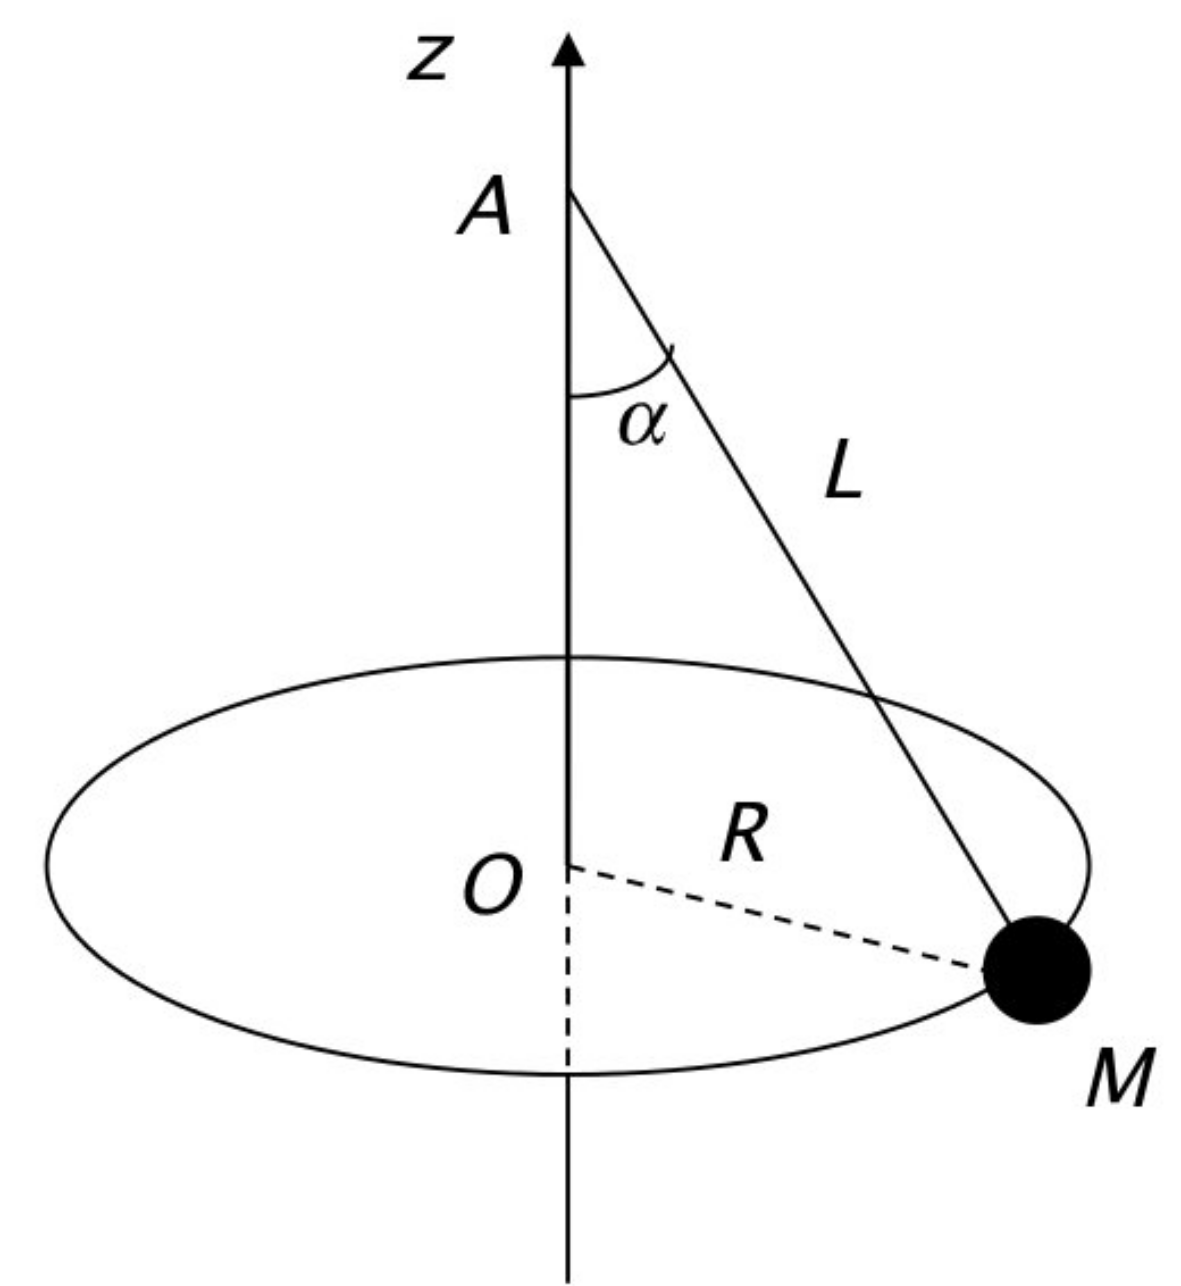
\includegraphics[width=\linewidth]{pendule_conique-plain}
		\end{center}
	\end{minipage}
}
\QR{%
	Effectuer un bilan des forces s'appliquant à la masse et les écrire
	dans la base choisie.
}{%
	\begin{itemize}[label=$\diamond$, leftmargin=10pt]
		\bitem{Système~:} \{M\} masse $m$
		\bitem{Référentiel~:} $\Rc\ind{labo}$ supposé galiléen
		\bitem{Repère~:} $(\Or, \ur, \ut, \uz)$ (voir schéma)
	\end{itemize} \smallbreak
	\begin{minipage}{0.65\linewidth}
		\begin{itemize}[label=$\diamond$, leftmargin=10pt]
			\bitem{Repérage~:} $R = \cte\Ra\dot{R} = 0$, $\tp = \w =
				\cte\Ra\dot{\w} = 0$~:
			\begin{align*}
				\OM       & = R\ur = L\sin\a\ur \\
				\vf_{\Mr} & = L\tp\sin\a\ut     \\
				          & = L\w\sin\a\ut      \\
				\af_{\Mr} & = -L\w^2\sin\a\ur
			\end{align*}
			\bitem{BDF~:}
			\[
				\begin{array}{ll}
					\textbf{Poids}   & \Pf = m\gf = -mg\uz             \\
					\textbf{Tension} & \Tf = T(-\sin\a\ur + \cos\a\uz)
				\end{array}
			\]
		\end{itemize}
	\end{minipage}
	\hfill
	\begin{minipage}{0.30\linewidth}
		\begin{center}
			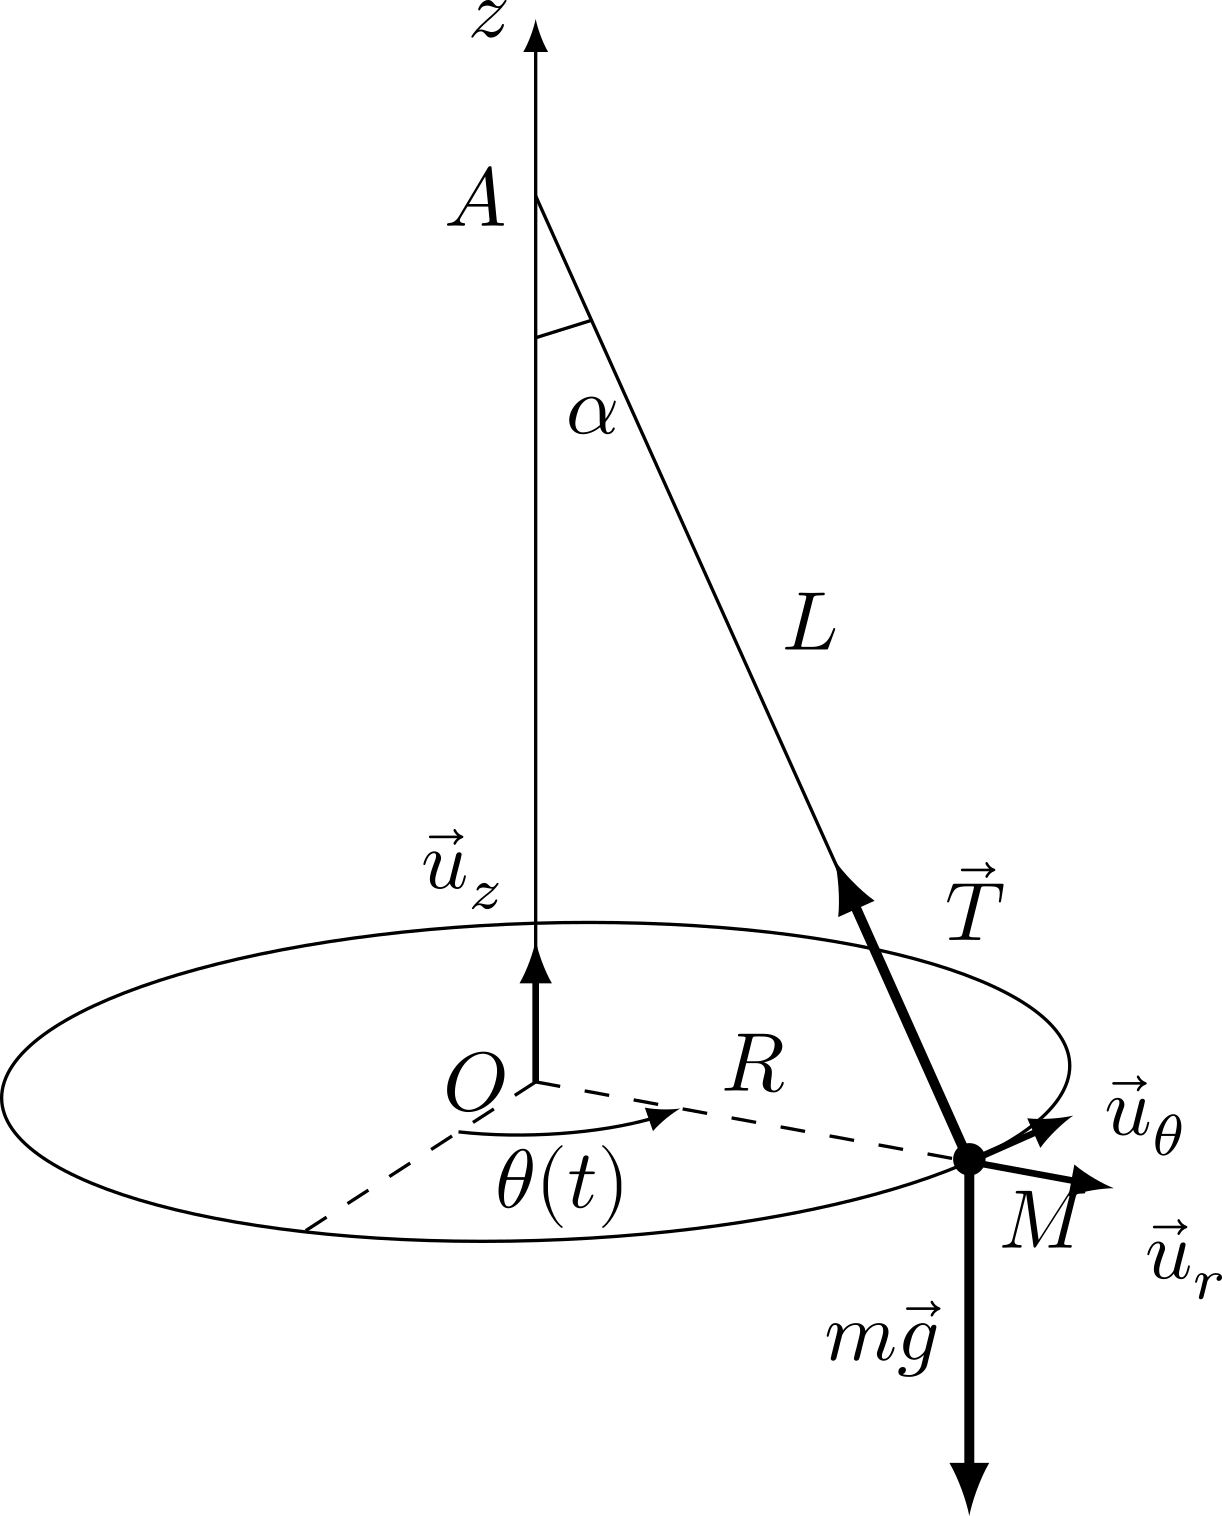
\includegraphics[width=\linewidth]{pendule_corr}
		\end{center}
	\end{minipage}
}
\QR{%
	Appliquer le PFD puis exprimer $\cos\a$ en fonction de $g$, $L$ et
	$\w$. En déduire que la vitesse angulaire doit forcément être supérieure
	à une vitesse angulaire limite $\w_{\lim}$ pour qu'un tel mouvement
	puisse être possible.
}{%
	On applique le PFD~:
	\begin{gather*}
		m\af = \Pf + \Tf
		\Lra
		\left\{
		\begin{aligned}
			-mL\w^2\cancel{\sin\a} & = -T\cancel{\sin\a} \\
			0                      & = T\cos\a -mg
		\end{aligned}
		\right.
		\Lra
		\left\{
		\begin{aligned}
			T & = mL\w^2            \\
			T & = \frac{mg}{\cos\a}
		\end{aligned}
		\right.
		\shortintertext{Soit}
		mL\w^2 = \frac{mg}{\cos\a}
		\Lra
		\boxed{\cos\a = \frac{g}{L\w^2}}
	\end{gather*}
	Pour que ce mouvement soit possible, il faut que $\cos\a < 1$, soit
	\begin{gather*}
		\frac{g}{L\w^2} < 1
		\Lra
		\boxed{\w \geq \sqrt{\frac{g}{L}} = \w_{\lim}}
	\end{gather*}
}
\QR{%
	Que dire du cas où $\w$ devient très grande~?
}{%
	Si $\w \gg \w_{\lim}$, alors $\cos\a \xrightarrow[\w \gg \w_{\lim}]{} 0$
	donc \fbox{$\a\xrightarrow[\w \gg \w_{\lim}]{} \pi/2$}~: le mouvement
	devient simplement circulaire, et se fait dans le plan horizontal
	contenant A.
}
\QR{%
	Application numérique~: calculer $\a$ pour $L = \SI{20}{cm}$ et $\w =
		\SI{3}{tours.s^{-1}}$.
}{%
	\leftcenters{On trouve}{\fbox{$\cos\a = \num{0.138} \Lra \a =
				\ang{82}$}}
}

\end{document}
